%%%%%%%%%%%%%%%%%%%%%%%%%%%%%%%%%%%%%%%%%%%%%%%%%%%%%%%%%%%%%
%% Begin exercise %%
%%%%%%%%%%%%%%%%%%%%%%%%%%%%%%%%%%%%%%%%%%%%%%%%%%%%%%%%%%%%%
\ex{Step-down converter and power loss calculation}


%%%%%%%%%%%%%%%%%%%%%%%%%%%%%%%%%%%%%%%%%%%%%%%%%%%%%%%%%%%%%
%% Task 1: Step-down converter without output filter %%
%%%%%%%%%%%%%%%%%%%%%%%%%%%%%%%%%%%%%%%%%%%%%%%%%%%%%%%%%%%%%

\task{Step-down converter without output filter}

A switching transistor is used for low-loss and stepless control of a car's rear window heating.
By varying the duty cycle of the transistor the average value of the heating power can be adjusted. The voltage in the car's electrical system is assumed to be constant with $U_1 = \SI{14}{\volt}$. The heater is dimensioned in such a way
that at its nominal voltage $ U_{\mathrm{2N}} = \SI{14}{\volt}$ it consumes a power of $ P_{\mathrm{LN}} = \SI{500}{\watt}$ and
can be modeled with an ohmic resistor. This circuit is shown in the figure \ref{fig:transistor circuit}.

\begin{figure}[h]
\begin{center}
    \begin{circuitikz}[european currents,european resistors,american inductors]
        \draw
        (0,0) coordinate(N1) to [short,-] ++(1.5,0) coordinate(U1p)
        ++(2,0) node[nigfete,rotate=90](Trans){}
        (U1p) to [short,i=$i_1(t)$] (Trans.drain)
        (Trans.source) to [short,-,i=$i_2(t)$] ++(1.5,0) coordinate(U2p)
        to [short,-] ++(1,0) to [R,l^=$R_\text{L}$, v_=$u_2$=straight] ++(0,-3) to [short,-] ++(-1,0) coordinate(U2n) to [short,-] (1,-3) coordinate(U1n) to [short,-] ++(-1,0) coordinate(N10)
         (N1) to [V] (N10)
         (0,0) to [V,v_=$U_1$] (0,-3)
       %  (U2p) to [open=straight,v^=$u_2(t)$] (U2n)
         (Trans.gate) to [short,-] ++(0,-.3) to [sqV] ++(0,-1) 
         (Trans.gate) ++(-0.3,0) node(T1){$\text{T}_\text{1}$}
      %   (Lp) to [V, v^=$U_2$] (Lp10)         
        ;
    \end{circuitikz}
\end{center}
\caption{Circuit with one transistor and one load resistor.}
    \label{fig:transistor circuit}
\end{figure}

%\begin{enumerate}
	\subtask{Draw qualitative current and voltage curves on the load resistor.}
        \begin{solutionblock}
            The graph \ref{fig:Currents and voltages during the period} shows the voltages and currents at the load resistor with the period $T_{\mathrm{s}}$, the switch-on time $T_{\mathrm{on}}$ and the switch-off time $T_{\mathrm{off}}$. 
        \begin{solutionfigure}[htb]
\begin{center}
      \begin{tikzpicture}
        \begin{axis}[
            domain=0:15,
            xmin=0, xmax=15,
            ymin=-1, ymax=2.5,
            samples=500,
            axis y line=center,
            axis x line=middle,
            xtick distance=1,
            ytick distance=2,
            extra y ticks=0,
            x label style={at={(axis description cs:1,0.25)},anchor=north},
            y label style={at={(axis description cs:0,.95)},anchor=south},
            width=0.8\textwidth,
            height=0.25\textwidth,
            xlabel={$t$},
            ylabel={{\color{blue}$u_\text{2}(t)$}\quad{\color{red}$i_\text{2}(t)$}},
            xtick={0},
            xticklabels={$0$},
            ytick={0,1,2},
            yticklabels={0,{\color{red}$\frac{U_1}{R_\text{L}}$},{\color{blue}$U_1$}},
            grid=none,
            grid style={line width=.1pt, draw=gray!10},
            major grid style={line width=.2pt,draw=gray!50},    ]
            \addplot[color=red,mark=none,solid] coordinates{
                (0, 0)
                (1, 0)
                (1, 1)
                (3, 1)
                (3, 0)
                (6, 0)
                (6, 1)
                (8, 1)
                (8, 0)
                (11, 0)
                (11, 1)
                (13, 1)
                (13, 0)
                (15, 0)
            };
            \addplot[color=blue,mark=none,dashed] coordinates{
                (0, 0)
                (1, 0)
                (1, 2)
                (3, 2)
                (3, 0)
                (6, 0)
                (6, 2)
                (8, 2)
                (8, 0)
                (11, 0)
                (11, 2)
                (13, 2)
                (13, 0)
                (15, 0)
            };
        \draw[>=triangle 45, <->] (axis cs:1,0.7) -- (axis cs:3,0.7);
        \node[anchor=north] at (axis cs:2,0.7){$T_\text{on}$};
        \draw[>=triangle 45, <->] (axis cs:3,0.7) -- (axis cs:6,0.7);
        \node[anchor=north] at (axis cs:4.5,0.7){$T_\text{off}$};
        \draw[>=triangle 45, <->] (axis cs:1,-0.3) -- (axis cs:6,-0.3);
        \node[anchor=north] at (axis cs:3.5,-0.3){$T_\text{s}$};
        \end{axis}
    \end{tikzpicture}
    % 
    %  \psfrag{u_L(t)}{$\textcolor{blue}{\mi uL (t)}$}
    %  	\psfrag{i_L(t)}{$\textcolor{red}{\mi iL (t)}$}
    %  	\psfrag{U1}{$\textcolor{blue}{U_1}$}
    %  	\psfrag{U1/R_L}[r][r]{$\textcolor{red}{\frac{U_1}{\mi RL}}$}
    %   	\includegraphics{bilder/loesung1_1.eps}
     \end{center}
     \caption{Display of currents and voltages depending on the switching phases.}
    \label{fig:Currents and voltages during the period}
\end{solutionfigure}
            
\end {solutionblock}

\subtask{ Draw the time curve of the instantaneous power at the load resistor.}


\begin {solutionblock}
The graph \ref{fig:Instantaneous power} shows the time curve of the instantaneous power at the load resistor.
\begin{solutionfigure}[h]
\begin{center}
    \begin{tikzpicture}
       \begin{axis}[
           domain=0:15,
           xmin=0, xmax=15,
           ymin=-1, ymax=2.5,
           samples=500,
           axis y line=center,
           axis x line=middle,
           xtick distance=1,
           ytick distance=2,
           extra y ticks=0,
           x label style={at={(axis description cs:1,0.25)},anchor=north},
           y label style={at={(axis description cs:-.05,.97)},anchor=south},
           width=0.8\textwidth,
           height=0.25\textwidth,
           xlabel={$t$},
           ylabel={{\color{blue}$p(t)$}},
           xtick={0},
           xticklabels={$0$},
           ytick={0,2},
           yticklabels={0,{\color{blue}$\frac{U_1^2}{R_L}$}},
           grid=none,
           grid style={line width=.1pt, draw=gray!10},
           major grid style={line width=.2pt,draw=gray!50},    ]
           \addplot[color=blue,mark=none,solid] coordinates{
               (0, 0)
               (1, 0)
               (1, 2)
               (3, 2)
               (3, 0)
               (6, 0)
               (6, 2)
               (8, 2)
               (8, 0)
               (11, 0)
               (11, 2)
               (13, 2)
               (13, 0)
               (15, 0)
           };
       \draw[>=triangle 45, <->] (axis cs:1,0.7) -- (axis cs:3,0.7);
       \node[anchor=north] at (axis cs:2,0.7){$T_\text{on}$};
       \draw[>=triangle 45, <->] (axis cs:3,0.7) -- (axis cs:6,0.7);
       \node[anchor=north] at (axis cs:4.5,0.7){$T_\text{off}$};
       \draw[>=triangle 45, <->] (axis cs:1,-0.3) -- (axis cs:6,-0.3);
       \node[anchor=north] at (axis cs:3.5,-0.3){$T_\text{s}$};
       \end{axis}
   \end{tikzpicture}
   % 
   %  	\psfrag{p(t)}{$\textcolor{blue}{p(t)}$}
   %  	\psfrag{U1^2/R}[r][r]{$\textcolor{blue}{\frac {U_1^2}{R}}$}
   %   	\includegraphics{bilder/loesung1_2.eps}
    \end{center}
   \caption{Instantaneous power at the load resistor.}
   % \ref{fig:Instantaneous power}
    \label{fig:Instantaneous power}
\end{solutionfigure}

\end{solutionblock}

\subtask{ Derive the relationships for the mean voltage $\overline u_2$, the mean current $\overline i_2$ and the mean power $P_{\mathrm{2}}$}.

\begin{solutionblock}
    In order to calculate the average voltage $\overline u_2$, the voltage $u_{\mathrm{2}}(t)$ must be integrated over the period $T_{\mathrm{s}}$.

    \begin{equation}
    \overline u_2 = \frac{1}{T_{\mathrm{s}}} \int_0^{ T_{\mathrm{s}}} u_2 (t) \, \mathrm{d}t = \frac{1}{ T_{\mathrm{s}}} \int_0^{D T_{\mathrm{s}}} U_1 \, \mathrm{d}t + \frac{1}{ T_{\mathrm{s}}} \int_{D  T_{\mathrm{s}}}^{ T_{\mathrm{s}}} 0 \, \mathrm{d}t$$
 $$= \left . \frac{U_1}{ T_{\mathrm{s}}} t \right |_0^{D  T_{\mathrm{s}}}  + 0 = \frac{U_1 D  T_{\mathrm{s}}}{ T_{\mathrm{s}}} = U_1 D
    \end{equation}

    In order to calculate the mean value $\overline i_2$, the current $i_{\mathrm{2}}(t)$ must be integrated over the period $T_{\mathrm{s}}$.
    \begin{equation}
 \overline i_2 = \frac{1}{ T_{\mathrm{s}}} \int_0^{ T_{\mathrm{s}}} i_2(t) \, \mathrm{d}t = \frac{1}{ T_{\mathrm{s}}}\int_0^{D  T_{\mathrm{s}}} \frac{U_1}{ R_{\mathrm{L}}} \, \mathrm{d}t + \frac{1}{ T_{\mathrm{s}}}\int_{D  T_{\mathrm{s}}}^{ T_{\mathrm{s}}} 0 \, \mathrm{d}t$$
 $$= \left . \frac{U_1}{ R_{\mathrm{L}}  T_{\mathrm{a}}}  t \right |_0^{D  T_{\mathrm{s}}} = \frac{U_1 D  T_{\mathrm{s}}}{ R_{\mathrm{L}}  T_{\mathrm{s}}} = \frac{U_1}{ R_{\mathrm{L}}} D
    \end{equation}

    In order to calculate the mean value $P_{\mathrm{2}}$, the power $p(t)$ must be integrated over the period $T_{\mathrm{s}}$.
    \begin{equation}
P_2 = \frac{1}{T_{\mathrm{s}}} \int_0^{T_{\mathrm{s}}} p(t) \mathrm{d}t = \frac{1}{T_{\mathrm{s}}} \int_0^{D T_{\mathrm{s}}} \frac{U_1^2}{ R_{\mathrm{L}}} \mathrm{d}t = \frac{U_1^2 D T_{\mathrm{s}}}{ T_{\mathrm{s}}  R_{\mathrm{L}}} = \frac{U_1^2 D}{ R_{\mathrm{L}}}
    \end{equation}
 
\end{solutionblock}
	% power $P_2$ as a function of the duty cycle $D$.


\subtask{ How large should the duty cycle D be selected so that an average voltage of $\overline u_2 = \SI{8}{\volt}$ is applied to the heater? What is the mean value of the current $\overline i_2$? What power $P_2$ converted into heat?}
\begin {solutionblock}

To determine the duty cycle D, the average voltage $\overline u_2$  must be divided by the source voltage $U_1$.
\begin{equation}
    \overline u_2 = D U_1 \Leftrightarrow D = \frac{\overline u_2}{U_1} = \frac{8\ \si{V}}{14 \ \si{V}}=0.57
\end{equation}
    
In order to determine the average current $\overline i_2$, the load resistance $R_{\mathrm{L}}$ must first be determined.
\begin{equation}
   \overline i_2 = \frac{U_1}{ R_{\mathrm{L}}}  D
\end{equation}

The known power equation is used to determine the load resistance $R_{\mathrm{L}}$.
\begin{equation}
   \quad  P_{\mathrm{LN}} = \frac{{ U_{\mathrm{2N}}}^2}{ R_{\mathrm{L}}} 
 \Leftrightarrow  R_{\mathrm{L}} = \frac{ U_{\mathrm{2N}}^2}{ P_{\mathrm{LN}}} = \frac{(14\ \si{V})^2}{500\ \si{W}} = \SI{392}{\mohm}
\end{equation}

This value can be used to determine the average current $\overline i_2$.
 $$\Rightarrow \overline i_2 = \frac{14\ \si{V}}{392\ \si{\mohm}} 0.57 =  \SI{20.36}{\ampere}$$
 
 To determine the power $P_2$ that is converted into heat, the corresponding duty cycle D must be considered!
 \begin{equation}
 P_2 = \frac{U_1^2}{ R_{\mathrm{L}}}  D = \frac{14\ \si{V}^2}{392\ \si{\mohm}}  0.57 = \SI{285}{\watt}
\end{equation}
\end{solutionblock}
	
\subtask{ When starting the engine, the heater may draw a maximum average current ${\overline i_{\mathrm{an}}} = \SI{10}{\ampere}$ from the
draw from the vehicle electrical system. With which duty cycle $D$ should the transistor be switched in this case?
What is the average voltage $\overline u_2$ at the heater? What power $P_2$ is converted into heat?}

%\frac{8\ \si{V}}{14 \ \si{V}}=0.57$$

\begin{solutionblock}

    Due to the structure of the circuit, it is noticeable that the average current $\overline i_1$ is equal to the average current $\overline i_2$. The corresponding ratio for $\overline i_{\mathrm{an}}$ can be calculated from this.
\begin{equation}
\overline i_1 = \overline i_2 = \frac{U_1}{ R_{\mathrm{L}}}  D \overset ! \leq {\overline i_{\mathrm{an}}}$$
 $$\Leftrightarrow D \leq \frac{ {\overline i_{\mathrm{an}}}  R_{\mathrm{L}}}{U_1} = \frac{10 \ \si{A} \cdot {392\ \si{\mohm}}} {14\ \si{V}} = 0.28
\end{equation}

To determine the average voltage $\overline u_2$ at the heater, the duty cycle D is offset against the source voltage $U_1$.
 \begin{equation}
 \overline u_2 = D  U_1 = 0.28 \cdot \SI{14}{\volt} = \SI{3.92}{\volt}
\end{equation}

To determine the power $P_2$ that is converted into heat, the corresponding duty cycle D must be considered!
 \begin{equation}
 P_2 = \frac{U_1^2 D}{ R_{\mathrm{L}}} = \frac{(14\ \si{V})^2 \cdot 0.28}{392\ \si{\mohm}}= \SI{140}{\watt}   
\end{equation}
\end{solutionblock}

\subtask{During the journey, the heat output should be $ P_{2f} = \SI{200} {\watt}$. How is the duty cycle
	 $D$ set? What are the mean values of the current $\overline i_2$ and the voltage $\overline u_2$?.}
     \begin{solutionblock}
        To determine the duty cycle D, the familiar power formula is used and the parameters are then applied.
  \begin{equation}
P_{2f} \overset ! = \frac{U_1^2}{ R_{\mathrm{L}}} D
 \Leftrightarrow D = \frac{ R_{\mathrm{L}}  P_{2f}}{U_1^2} = \frac{{392\ \si{\mohm}} \cdot 200 \ \si{W}}{(14\ \si{V})^2} = 0.4
\end{equation}
The known equations are used to determine the average current $\overline i_2$ and the average voltage $\overline u_2$.
 \begin{equation}
 \overline i_2 = \frac{U_1}{ R_{\mathrm{L}}} D = \frac{\SI{14}{\volt}}{392\ \si{\mohm}} \cdot 0.4 = \SI{14.29}{\ampere}
\end{equation}
\begin{equation}
 \overline u_2 = U_1 D = {\SI{14}{\volt}} \cdot 0.4 = \SI{5.6}{\volt}
\end{equation}
\end{solutionblock}

%%%%%%%%%%%%%%%%%%%%%%%%%%%%%%%%%%%%%%%%%%%%%%%%%%%%%%%%%%%%%
%% Task 2: Step-down converter with output filter %%
%%%%%%%%%%%%%%%%%%%%%%%%%%%%%%%%%%%%%%%%%%%%%%%%%%%%%%%%%%%%%

\task{Step-down converter with output filter}
A step-down converter is used to charge a mobile phone from the vehicle electrical system with the vehicle electrical system voltage $U_1 = \SI{13.5}{\volt}$. The input voltage of the mobile phone is $U_2 = \SI{4.5}{\volt}$.
\begin{center}
\begin{circuitikz}[european currents,european resistors,american inductors]
	\draw
	(0,0) coordinate(U+) to [short,-] ++(0.5,0)  
	node[currarrow](Tl){} -- ++(1,0) ++(0.5,0) node[nigfete,rotate=90](Trans){} -- ++(1.5,0) coordinate(Tr)  to [short,-*] ++(0.5,0) coordinate(junc1)   -- ++(0.5,0) coordinate(Ll) to [L,l_=$L$,i^=$i_\text{L}$] ++(2,0) coordinate(Lr) to [short,-*] ++(0.5,0) coordinate(junc2)  -- ++(2,0)  coordinate(Rt) to [R,l_=$R$,i_=$i_\text{2}$,v^=$U_\text{2}$,voltage shift=0.5] ++(0,-3) coordinate(Rb) to [short,-*] ++(-2,0) coordinate(junc3) to [short,-*] ++(-3,0) coordinate(junc4) to [short] ++(-2,0) coordinate(junc5) to [short,-] ++(-2,0) coordinate(U-)
        (junc2) to [C,l_=$C$](junc3)
        (junc4) to [short]  ++(0,0.5) coordinate(Db) to[D-,l^=$D$]  ++(0,2) coordinate(Dt) to [short] (junc1)
         (Trans.G)  to [sqV] ++(0,-1)(junc5) 
	
	(U+) to [V=$U_1$] (U-)
	
  	(Trans)  node[anchor=south,color=black]{$T_1$}	
 	(Tl)  node[anchor=south,color=black]{$i_\text{1}$}	
	;
\end{circuitikz}
\end{center}

(both voltages are assumed to be constant). The inductance of the ideal coil is $L = \SI{10}{\milli\henry}$
The switching frequency is $f_s = \SI{ 100}{\kilo\hertz}$. All components are ideal.

\subtask{Draw the equivalent circuits for the two switching states.}
% Solution of subtask
\begin{solutionblock}
	\begin{tabular}{cc}
        	Transistor leitet & Diode leitet\\
       	\begin{circuitikz}[european currents,european resistors,american inductors,]
	        \draw
            (0,0) coordinate(u1o)
            to [V,v^=$U_2$] ++(0,-3) coordinate(u1u)
                (u1o) to [short,-,i^<=$i_2$] ++(-1,0) to [L,l_=$L$,v^<=$u_\text{L}$,mirror] ++(-3,0) to [short,-,i^<=$i_1$] ++(-1,0) coordinate(uqo)
                (u1u) to [short,-] ++(-5,0) coordinate(uqu)
                (uqo) to [V,v_=$U_1$] (uqu)
                ;
        \end{circuitikz}
&
      	\begin{circuitikz}[european currents,european resistors,american inductors,]
            \draw
            (0,0) coordinate(u2o)
            to [V,v^=$U_2$] ++(0,-3) coordinate(u2u)
                (u2o) to [short,-,i^<=$i_2$] ++(-1,0) to [L,l_=$L$,v^<=$u_\text{L}$,mirror] ++(-3,0) coordinate(Ll) ++(-1,0) coordinate(uqo)
                (u2u) to [short,-*] ++(-4,0) coordinate(Llu) to [short,-] ++(-1,0) coordinate(uqu)
                (Llu) to [short,-,i_=$i_1$] (Ll)
                (uqo) to [V,v_=$U_1$] (uqu)
                ;
        \end{circuitikz}
% \\
%         	\psfrag {U1}{$U_1$}
% 		\psfrag {U2}{$U_2$}
% 		\psfrag {i1}{$i_1$}
% 		\psfrag {i2}{$i_2$}
% 		\psfrag {uL}{$u_L$}
% 		\psfrag {L}{$L$}
%         	\includegraphics{bilder/loesung2_1a} 
%         	& 
%         	\psfrag {U1}{$U_1$}
% 		\psfrag {U2}{$U_2$}
% 		\psfrag {i1}{$i_1$}
% 		\psfrag {i2}{$i_2$}
% 		\psfrag {uL}{$u_L$}
% 		\psfrag {L}{$L$}
%         	\includegraphics{bilder/loesung2_1b}
	\end{tabular}

\end{solutionblock}

\subtask{At what duty cycle $D$ should the buck converter be operated?}
% Solution of subtask

\begin{solutionblock}
    \begin{equation}
        D = \frac{U_2}{U_1} = \frac{\SI{ 4.5}{\volt}}{\SI{ 13.5}{\volt}} = \frac{1}{3}
    \end{equation}

\end{solutionblock}
   
\subtask{Qualitatively draw the voltage and current waveforms in the components.}
% Solution of subtask

\begin{solutionblock}    
    \begin{center}
        \definecolor{orange}{rgb}{1.0,0.5,0}
        \begin{tikzpicture}
            \begin{groupplot}[group style={%
                group size=1 by 5,
            %     group name=plots,
                xlabels at=edge bottom,
                y descriptions at=edge left,
                },
            %     ybar,
                xmin=0, xmax=13.5,
                domain=0:13,
            %     enlarge x limits={abs=.5},
                width=0.6\textwidth,
            %     height=0.6\textwidth,
            %     scaled y ticks=base 10:-3,
            %     xticklabels from table={\first}{Criterion},
            %     x tick label style={rotate=90,anchor=east},
            %     xtick=data,
            %         x label style={at={(axis description cs:1,0)},anchor=north},
            %         xlabel={$t$},
                    xtick={0,1,4,5,8,9,12,13},
                    xticklabels={{},{},{},{},{},{},{},{},{},{}},
                    grid=both,
                    grid style={line width=.1pt, draw=gray!10},
                    major grid style={line width=.2pt,draw=gray!50},    
                    axis y line=center,
                    axis x line=middle,
                    ]
            
            %     ]
            
            
            \nextgroupplot[
            %         domain=0:13,
            %         xmin=0, xmax=13.5,
                    ymin=0, ymax=1.2,
                    samples=500,
            %         axis y line=center,
            %         axis x line=middle,
            %         xtick distance=1,
                    ytick distance=2,
                    extra y ticks=0,
                    x label style={at={(axis description cs:1,0)},anchor=north},
                    y label style={at={(axis description cs:-.05,.97)},anchor=south},
            %         width=0.6\textwidth,
                    height=0.2\textwidth,
                    xlabel={$t$},
                    ylabel={{\color{orange}$u_\text{T}$}},
            %         xtick={0,1,4,5,8,9,12,13},
            %         xticklabels={$0$,{},{},{},{},{},{},{},{},{}},
                    ytick={0,1},
                    yticklabels={0,$U_1$},
            %         grid=both,
            %         grid style={line width=.1pt, draw=gray!10},
            %         major grid style={line width=.2pt,draw=gray!50},    
            ]
                    \addplot[color=orange,mark=none,solid] coordinates{
                        (0, 0)
                        (1, 0)
                        (1, 1)
                        (4, 1)
                        (4, 0)
                        (5, 0)
                        (5, 1)
                        (8, 1)
                        (8, 0)
                        (9, 0)
                        (9, 1)
                        (12,1)
                        (12,0)
                        (13, 0)
                    };  
                    
            \nextgroupplot[
            %         domain=0:13,
            %         xmin=0, xmax=13.5,
                    ymin=0, ymax=1.2,
                    samples=500,
                    axis y line=center,
            %         axis x line=middle,
            %         xtick distance=1,
                    ytick distance=2,
                    extra y ticks=0,
                    x label style={at={(axis description cs:1,0)},anchor=north},
                    y label style={at={(axis description cs:-.05,.97)},anchor=south},
            %         width=0.6\textwidth,
                    height=0.2\textwidth,
                    xlabel={$t$},
                    ylabel={{\color{blue}$u_\text{D}$}},
            %         xtick={0,1,4,5,8,9,12,13},
            %         xticklabels={$0$,{},{},{},{},{},{},{},{},{}},
                    ytick={0,.33,1},
                    yticklabels={0,$U_2$,$U_1$},
            %         grid=both,
            %         grid style={line width=.1pt, draw=gray!10},
            %         major grid style={line width=.2pt,draw=gray!50},    
            ]
                    \addplot[color=blue,mark=none,solid] coordinates{
                        (0, 1)
                        (1, 1)
                        (1, 0)
                        (4, 0)
                        (4, 1)
                        (5, 1)
                        (5, 0)
                        (8, 0)
                        (8, 1)
                        (9, 1)
                        (9, 0)
                        (12,0)
                        (12,1)
                        (13, 1)
                        (13, 0)
                    };
                
            \nextgroupplot[
            %         domain=0:13,
            %         xmin=0, xmax=13.5,
                    ymin=-.5, ymax=1.2,
                    samples=500,
                    axis y line=center,
            %         axis x line=middle,
            %         xtick distance=1,
                    ytick distance=2,
                    extra y ticks=0,
                    x label style={at={(axis description cs:1,0.25)},anchor=north},
                    y label style={at={(axis description cs:-.05,.97)},anchor=south},
            %         width=0.6\textwidth,
                    height=0.25\textwidth,
                    xlabel={$t$},
                    ylabel={{\color{orange}$u_\text{L}$}},
            %         xtick={0,1,4,5,8,9,12,13},
            %         xticklabels={$0$,{},{},{},{},{},{},{},{},{}},
                    ytick={-.333,0,1},
                    yticklabels={$-U_2$,0,$U_1-U_2$},
            %         grid=both,
            %         grid style={line width=.1pt, draw=gray!10},
            %         major grid style={line width=.2pt,draw=gray!50},    
            ]
                    \draw [fill=green] (axis cs:4,0) rectangle (axis cs:5,1);
                    \draw [fill=cyan] (axis cs:5,0) rectangle (axis cs:8,-.3333);
                    \addplot[color=orange,mark=none,solid] coordinates{
                        (0, 1)
                        (1, 1)
                        (1, -.333)
                        (4, -.333)
                        (4, 1)
                        (5, 1)
                        (5, -.333)
                        (8, -.333)
                        (8, 1)
                        (9, 1)
                        (9, -.333)
                        (12, -.333)
                        (12, 1)
                        (13, 1)
                        (13, -.333)
                    };
                \node[anchor=center] at (axis cs:4.5,0.5){\tiny $ A_\text{ein}$};
                \node[anchor=center] at (axis cs:6.5,-0.1667){\tiny $ A_\text{aus}$};
            
            \nextgroupplot[
            %         domain=0:13,
            %         xmin=0, xmax=13.5,
                    ymin=0, ymax=1.2,
                    samples=500,
                    axis y line=center,
            %         axis x line=middle,
            %         xtick distance=1,
                    ytick distance=2,
                    extra y ticks=0,
                    x label style={at={(axis description cs:1,0)},anchor=north},
                    y label style={at={(axis description cs:-.05,.97)},anchor=south},
            %         width=0.6\textwidth,
                    height=0.2\textwidth,
                    xlabel={$t$},
                    ylabel={{\color{red}$i_\text{L}$}},
            %         xtick={0,1,4,5,8,9,12,13},
            %         xticklabels={$0$,{},{},{},{},{},{},{},{},{}},
                    ytick={0,.5,.75,1},
                    yticklabels={0,,,},
            %         grid=both,
            %         grid style={line width=.1pt, draw=gray!10},
            %         major grid style={line width=.2pt,draw=gray!50},    
            ]
                    \addplot[color=red,mark=none,solid] coordinates{
                        (0, 0.5)
                        (1, 1)
                        (4, 0.5)
                        (5, 1)
                        (8, 0.5)
                        (9, 1)
                        (12,0.5)
                        (13,1)
                    };
            
            \nextgroupplot[
            %         domain=0:13,
            %         xmin=0, xmax=13.5,
                    ymin=0, ymax=1.2,
                    samples=500,
                    axis y line=center,
            %         axis x line=middle,
            %         xtick distance=1,
                    ytick distance=2,
                    extra y ticks=0,
                    x label style={at={(axis description cs:1,0)},anchor=north},
                    y label style={at={(axis description cs:-.0,.97)},anchor=south},
            %         width=0.6\textwidth,
                    height=0.2\textwidth,
                    xlabel={$t$},
                    ylabel={{\color{orange}$i_\text{T}$}\quad{\color{blue}$i_\text{D}$}},
            %         xtick={0,1,4,5,8,9,12,13},
            %         xticklabels={$0$,{},{},{},{},{},{},{},{},{}},
                    ytick={0,.5,.75,1},
                    yticklabels={0,,,},
            %         grid=both,
            %         grid style={line width=.1pt, draw=gray!10},
            %         major grid style={line width=.2pt,draw=gray!50},    
            ]
                    \addplot[color=orange,mark=none,solid] coordinates{
                        (0,0)
                        (0, 0.5)
                        (1, 1)
                        (1, 0)
                        (4,0)
                        (4,0.5)
                        (5, 1)
                        (5,0)
                        (8,0)
                        (8, 0.5)
                        (9, 1)
                        (9,0)
                        (12,0)
                        (12,0.5)
                        (13,1)
                        (13,0)
                    };
                    \addplot[color=blue,mark=none,solid] coordinates{
                        (1,1)
                        (4, 0.5)
                    };
                    \addplot[color=blue,mark=none,solid] coordinates{
                        (5,1)
                        (8, 0.5)
                    };
                    \addplot[color=blue,mark=none,solid] coordinates{
                        (9,1)
                        (12, 0.5)
                    };
                    \addplot[color=blue,mark=none,solid] coordinates{
                        (0,0)
                        (1, 0)
                    };
                    \addplot[color=blue,mark=none,solid] coordinates{
                        (4,0)
                        (5,0)
                    };
                    \addplot[color=blue,mark=none,solid] coordinates{
                        (8,0)
                        (9,0)
                    };
                    \addplot[color=blue,mark=none,solid] coordinates{
                        (12,0)
                        (13,0)
                    };
                    \addplot[color=blue,mark=none,dashed] coordinates{
                        (1,0)
                        (1,1)
                    };
                    \addplot[color=blue,mark=none,dashed] coordinates{
                        (4,0)
                        (4,0.5)
                    };
                    \addplot[color=blue,mark=none,dashed] coordinates{
                        (5,0)
                        (5,1)
                    };
                    \addplot[color=blue,mark=none,dashed] coordinates{
                        (8,0)
                        (8,0.5)
                    };
                    \addplot[color=blue,mark=none,dashed] coordinates{
                        (9,0)
                        (9,1)
                    };
                    \addplot[color=blue,mark=none,dashed] coordinates{
                        (12,0)
                        (12,0.5)
                    };
                    \addplot[color=blue,mark=none,dashed] coordinates{
                        (13,0)
                        (13,1)
                    };
            
            \end{groupplot}
        \end{tikzpicture}
        
    
    % 		\psfrag{U1}{$U_1$}
    % 		\psfrag{U2}{$U_2$}
    %  		\psfrag{UT}{$\textcolor{orange}{\mi UT}$}
    % 		\psfrag{UL}{$\textcolor{orange}{\mi UL}$}
    % 		\psfrag{UD}{$\textcolor{blue}{\mi UD}$}
    % 		\psfrag{IT}{$\textcolor{orange}{\mi IT}$}
    % 		\psfrag{IL}{$\textcolor{red}{\mi IL}$}
    % 		\psfrag{ID}{$\textcolor{blue}{\mi ID}$}
    % 		\psfrag{Aein}{$\mi A{ein}$}
    % 		\psfrag{Aaus}{$\mi A{aus}$}
    % 		\includegraphics[width =8cm]{bilder/verlaeufe_aufg_2.eps}
    \end{center}
    
    
\end{solutionblock}

\subtask{How large is the current fluctuation range $\triangle i_L$ of the coil current in normal operation at a switching frequency of $f_s = \SI{ 100}{\kilo\hertz}$.}
% Solution of subtask
\begin{solutionblock}
    \begin{center}
        \begin{tikzpicture}
        \begin{axis}[
                domain=0:15,
                xmin=0, xmax=7,
                ymin=-1.5, ymax=2.5,
                samples=500,
                axis y line=center,
                axis x line=middle,
                xtick distance=1,
                ytick distance=2,
                extra y ticks=0,
                x label style={at={(axis description cs:1,0.33)},anchor=north},
                y label style={at={(axis description cs:-.05,.97)},anchor=south},
                width=0.8\textwidth,
                height=0.5\textwidth,
                xlabel={$t$},
                ylabel={$i_\text{L}$},
                xtick={0,2,5},
                xticklabels={$0$,{},{}},
                ytick={0,1,2},
                yticklabels={0,$\frac{\Delta i_\text{L}}{2}$,$\Delta i_\text{L}$},
                grid=both,
                grid style={line width=.1pt, draw=gray!10},
                major grid style={line width=.2pt,draw=gray!50},    ]
                \addplot[color=blue,mark=none,solid] coordinates{
                    (0, 0)
                    (2, 2)
                    (5, 0)
                    (7, 2)
                };
                \draw[>=triangle 45, <->] (axis cs:0,-.3) -- (axis cs:2,-.3);
                \node[anchor=north] at (axis cs:1,-.3){$D T_\text{s}$};
                \draw[>=triangle 45, <->] (axis cs:2,-.3) -- (axis cs:5,-.3);
                \node[anchor=north] at (axis cs:3.5,-.3){$(1-D) T_\text{s}$};
                \draw[>=triangle 45, <->] (axis cs:0,-1) -- (axis cs:5,-1);
                \node[anchor=north] at (axis cs:2.5,-1){$T_\text{s}$};
            \end{axis}
    \end{tikzpicture}
    % 
    % 		\psfrag{iL}{$\mi iL$}
    % 		\psfrag{delta iL}{$\triangle \mi iL$}
    % 		\psfrag{I2=delta iL/2}{$I_2 = \frac{\triangle \mi iL}{2}$}
    % 		\psfrag{DTs}{$D \mi Ts$}
    % 		\psfrag{(1-D)Ts}{$(1-D) \mi Ts$}
    % 		\psfrag{Ts}{$\mi Ts$}
    % 	 	\includegraphics{bilder/loesung2_4.eps}
    \end{center}
    \begin{equation}
        f_s = \SI{ 100}{\kilo\hertz} \Rightarrow T_s = \SI{ 10}{\micro\second} \Rightarrow T_e = D \cdot T_s = \frac{\SI{ 10}{\micro \second}}{3}
    \end{equation}
    \begin{equation}
        U_L = U_1 - U_2 = L \frac{d i_L}{dt} \overset {\begin{matrix}\text{Assumption of ideal coil}\\ \Rightarrow \text{linear current flow} \end{matrix}} = L \frac{\triangle i_L}{\triangle t} = L \frac{\triangle i_L}{T_e}
    \end{equation}
    \begin{equation}
        \Rightarrow \triangle i_L = \frac{U_1 - U_2}{L} T_e = \frac{\SI{13.5}{\volt} - \SI{4.5}{\volt}}{\SI{10}{\micro \henry} \cdot \frac{\SI{10}{\micro \second}}{3}} = \SI{3}{\ampere}
    \end{equation}
    \begin{equation}
        I_{2min} = \frac{\triangle i_L}{2} = \SI{1.5}{\ampere}
    \end{equation}
\end{solutionblock}

\subtask{When starting the engine, the input voltage drops to $U_{1min} = \SI{ 10}{\volt}$.
The voltage regulator of the buck converter changes the duty cycle so that the output voltage $U_2 = \SI{ 4.5}{\volt}$ is kept stable.
What duty cycle D is set?}
% Solution of subtask
\begin{solutionblock}
    \begin{equation}    
        D= \frac{U_2}{U_{1min}} = \frac{\SI{4.5}{\volt}}{\SI{10}{\volt}} = 0.45
    \end{equation}    
\end{solutionblock}

\subtask{Where is the boundary of discontinuous conduction mode?}
% Lösung des Unterpunktes
\begin{solutionblock}
    \begin{equation}
        \triangle i_L = \frac{U_{1min} - U_2}{L} D \cdot T_s = \frac{(\SI{10}{\volt} - \SI{4.5}{\volt}) \cdot 0.45 \cdot \SI{10}{\micro \second}}{\SI{10}{\micro \henry}} = \SI{2.475}{\ampere}
    \end{equation}
    \begin{equation}
        I_{2min} = \frac{\triangle i_L}{2} \approx \SI{1.24}{\ampere}
    \end{equation}
\end{solutionblock}

\subtask{In the next step, the input voltage is constant, and the output voltage is to be adjusted using the duty cycle.
         At what duty cycle $D$ will the peak-to-peak current ripple be maximal?}
% Lösung des Unterpunktes
\begin{solutionblock}
    \begin{equation}
        U_2 = D \cdot U_1
    \end{equation}
    \begin{equation}
        \triangle i_L (D) = \frac{U_1 - D \cdot U_1}{L} \cdot D \cdot T_s = \frac{U_1 T_s}{L} (D-D^2)
    \end{equation}
    \begin{equation}
        \triangle i_L' (D) \overset ! = 0 = \frac{U_1 T_s}{L}(1-2 D)
    \end{equation}
    \begin{equation}
        \Rightarrow 1 = 2 D \Rightarrow D = \frac{1}{2}
    \end{equation}
\end{solutionblock}
\subtask{Sketch the course of the current fluctuation width $\triangle i$ as a function of the duty cycle $D$.}
% Lösung des Unterpunktes
\begin{solutionblock}
    \begin{center}
        \begin{tikzpicture}
            \begin{axis}[
                domain=0:1,
                xmin=0, xmax=1.2,
                ymin=0, ymax=1.2,
                samples=500,
                axis y line=center,
                axis x line=middle,
                xtick distance=0.5,
                ytick distance=2,
                extra y ticks=0,
                x label style={at={(axis description cs:1,0)},anchor=north},
                y label style={at={(axis description cs:-.05,.95)},anchor=south},
                width=0.6\textwidth,
                height=0.4\textwidth,
                xlabel={$D$},
                ylabel={$\Delta i_\text{L}$},
        %          xtick={0, 1},
        %         xticklabels={$0$,$\tau$},
                ytick={0,1},
                yticklabels={0,$\frac{U_1 T_s}{4L}$},
                grid=both,
                grid style={line width=.1pt, draw=gray!10},
                major grid style={line width=.2pt,draw=gray!50},    ]
                \addplot+[color=blue,mark=none]{1-((2*(x-0.5))^2)};
            \end{axis}
        \end{tikzpicture}

    % 	\psfrag{delta iL}{$\triangle \mi iL$}
    % 	\psfrag{(U1Ts)/(4L)}{$\frac{U_1 \mi Ts}{4L}$}
    % 	\psfrag{0}{$0$}
    % 	\psfrag{0.5}{$\frac{1}{2}$}
    % 	\psfrag{1}{$1$}
    % 	\psfrag{D}{$D$}
    % 	 	\includegraphics[width = 7cm]{bilder/loesung2_8.eps}
    \end{center}
\end{solutionblock}

%%%%%%%%%%%%%%%%%%%%%%%%%%%%%%%%%%%%%%%%%%%%%%%%%%%%%%%%%%%%%
%% Task 3: Power losses within the step-down converter %%
%%%%%%%%%%%%%%%%%%%%%%%%%%%%%%%%%%%%%%%%%%%%%%%%%%%%%%%%%%%%%


\task{Power losses within the step-down converter}
The power loss of a buck converter is to be analysed. The inductance is so large
that the current ripple in the output current can be neglected. $ i_{\mathrm{2}}(t) = I_{\mathrm{2}} =const $. Furthermore, the component values are given in \ref{table:Parameters of the circuit} and the currents and voltages of the switch-on and switch-off processes in \ref{fig:Switch-on behaviour and switch-off behaviour of} and \ref{fig:Switch-on behaviour and switch-off behaviour of voltage}. 

%\ref{fig:Currents and voltages during the period}

\begin{figure}[h]
    \begin{center}
        \begin{circuitikz}[european currents,european resistors,american inductors]
            \draw
        (0,0) coordinate(N1) to [short] ++(1.5,0) coordinate(Ud)
        ++(0,-1) node[nigfete](Trans){}
        (Ud) to [short,i=$i_{\mathrm{c}}(t)$] (Trans.drain)
        (Trans.source) to [short,-] ++(0,0) coordinate(U2p)
        node[circ]{}
        to [short,-] ++(0,0) to [L,l^=$L$] ++(3,0) coordinate(Lp) to [short,-] ++(0,-2) coordinate(Lp10)
        (Lp) to [V, v_=$U_2$] (Lp10)
        (Lp) to [open] (Lp10)
        coordinate(Lp10) to  [short,-] ++(-3,0) coordinate(D)
        to [D,l^=$D$, i=$i_{\mathrm{D}}(t)$] ++(0,2)
        (0,-3.77) coordinate(Bw) to [short] ++(3,0) coordinate(U1)
        %(N1) to [V] (Bw)
        (N1) to [V,v_=$U_1$] (Bw)
           ;
        \end{circuitikz}
    \end{center}
    \caption{Circuit buck converter.}
        \label{fig:Graphic of a buck converter}
    \end{figure}

    
      \begin{table}[h]
        \centering  % Zentriert die Tabelle
                \begin{tabular}{|l|l|l|l|}
            \hline
            \multicolumn{2}{|l|}{\textbf{DC link voltage:}} & \multicolumn{2}{l|}{\textbf{Diode:}} \\
            \hline
            \multicolumn{2}{|l|}{$U_{\mathrm{1}} = \SI{600}{\volt}$} & Forward voltage: & $u_{\mathrm{F}} = \SI{2.7}{\volt}$ \\
            \hline
            \multicolumn{2}{|l|}{Output current: $I_2 = 30$A} & Switch-on losses: & $E_{\text{on},D} = \SI{52}{\micro\joule}$ \\
            \hline
            \multicolumn{2}{|l|}{Clock frequency: $f_{\mathrm{T}} = \SI{25}{\kilo\hertz}$} & Switch-off losses: & $E_{\text{off},D} = \SI{240}{\micro\joule}$ \\
            \hline
            \multicolumn{2}{|l|}{\textbf{IGBT:}} & \multicolumn{2}{l|}{} \\
            \hline
            Forward voltage: & $u_{\mathrm{on},\mathrm{CE}} = \SI{2.5}{\volt}$ & \multicolumn{2}{l|}{} \\
            \hline
            \multicolumn{2}{|l|}{\textbf{Inductance:}} & \multicolumn{2}{l|}{} \\
            \hline
            Copper resistance: & $R_{\text{Cu}} = \SI{45}{\milli\ohm}$ & \multicolumn{2}{l|}{} \\
            \hline
            Iron losses: & $P_{\mathrm{l},\text{FE}} = \SI{13}{\watt}$ & \multicolumn{2}{l|}{} \\
            \hline
        \end{tabular}
        \caption{Parameters of the circuit.}  % Beschriftung der Tabelle
        \label{table:Parameters of the circuit}
    \end{table}

    \begin{figure}[h]
        \centering
        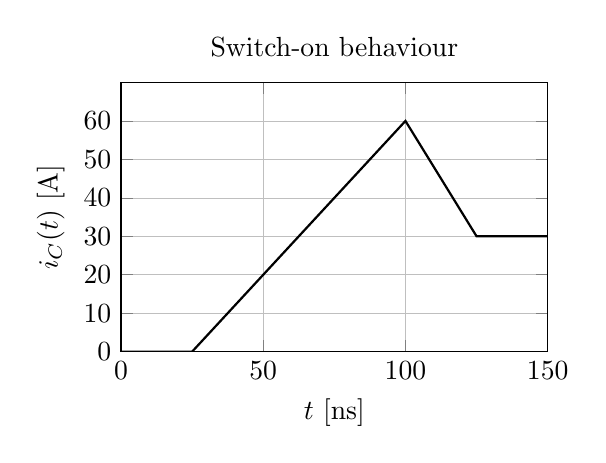
\begin{tikzpicture}
        \begin{axis}[
            width=7cm, height=5cm,
            grid=both,
            major grid style={line width=.2pt,draw=gray!50},
            minor grid style={line width=.1pt,draw=gray!20},
            xlabel={$t$ [ns]},
            ylabel={$i_C(t)$ [A]},
            title={Switch-on behaviour},
            xmin=0, xmax=150,
            ymin=0, ymax=70,
            xtick={0, 50, 100, 150},
            ytick={0, 10, 20, 30, 40, 50, 60},
            ]
            % Einschaltverhalten graph
            \addplot[
                thick,
                mark=none,
                color=black,
            ] coordinates {
                (0,0) (25,0) (50, 20) (75, 40) (100, 60) (125, 30) (150, 30)
            };
        \end{axis}
        \end{tikzpicture} 
        \hspace{1cm} % Abstand zwischen den beiden Diagrammen
        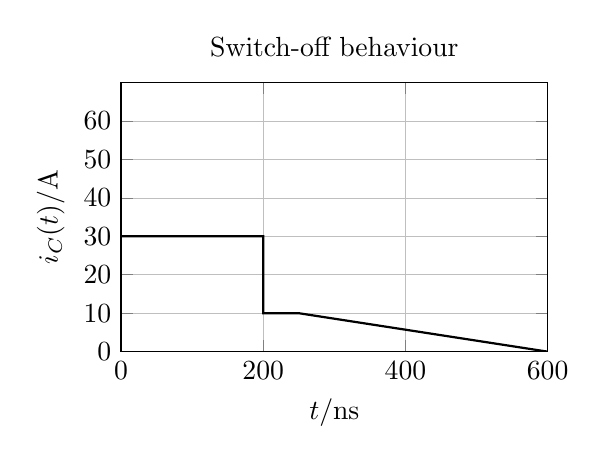
\begin{tikzpicture}
        \begin{axis}[
            width=7cm, height=5cm,
            grid=both,
            major grid style={line width=.2pt,draw=gray!50},
            minor grid style={line width=.1pt,draw=gray!20},
            xlabel={$t$/ns},
            ylabel={$i_C(t)$/A},
            title={Switch-off behaviour},
            xmin=0, xmax=600,
            ymin=0, ymax=70,
            xtick={0, 200, 400, 600},
            ytick={0, 10, 20, 30, 40, 50, 60},
            ]
            % Ausschaltverhalten graph
            \addplot[
                thick,
                mark=none,
                color=black,
            ] coordinates {
                (0,30) (200, 30) (200, 10) (250, 10) (600, 0)
            };
        \end{axis}
        \end{tikzpicture}
        \caption{Switch-on behaviour and switch-off behaviour of $i_{\mathrm{C}}(t)$}
        \label{fig:Switch-on behaviour and switch-off behaviour of}

    %    \end{figure}
       
  %  \begin{figure}[h]
     %   \centering
        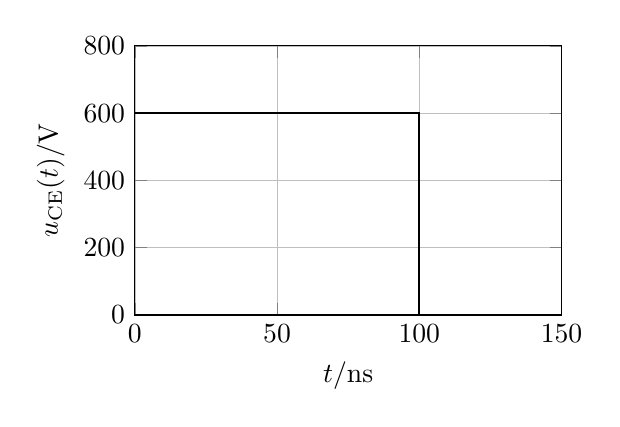
\begin{tikzpicture}
        \begin{axis}[
            width=7cm, height=5cm,
            grid=both,
            major grid style={line width=.2pt,draw=gray!50},
            minor grid style={line width=.1pt,draw=gray!20},
            xlabel={$t$/ns},
            ylabel={$u_{\mathrm{CE}}(t)$/V},
            xmin=0, xmax=150,
            ymin=0, ymax=800,
            xtick={0, 50, 100, 150},
            ytick={0,200, 400, 600, 800},
            ]
            % Einschaltverhalten graph
            \addplot[
                thick,
                mark=none,
                color=black,
            ] coordinates {
                (0,600) (100, 600) (100, 0)
            };
        \end{axis}
        \end{tikzpicture}
        \hspace{1cm} % Abstand zwischen den beiden Diagrammen
        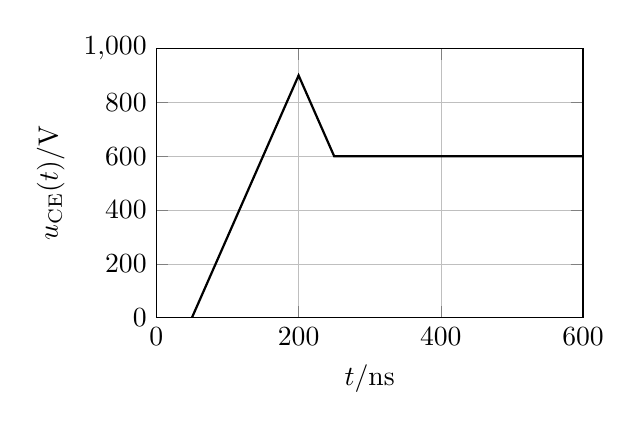
\begin{tikzpicture}
        \begin{axis}[
            width=7cm, height=5cm,
            grid=both,
            major grid style={line width=.2pt,draw=gray!50},
            minor grid style={line width=.1pt,draw=gray!20},
            xlabel={$t$/ns},
            ylabel={$u_{\mathrm{CE}}(t)$/V},
            xmin=0, xmax=600,
            ymin=0, ymax=1000,
            xtick={0,200, 400, 600},
            ytick={0,200, 400, 600,800, 1000},
            ]
            % Ausschaltverhalten graph
            \addplot[
                thick,
                mark=none,
                color=black,
            ] coordinates {
                (50,0) (200, 900) (250, 600) (600, 600)
            };
        \end{axis}
        \end{tikzpicture}
        \caption{Switch-on behaviour and switch-off behaviour of $u_{\mathrm{CE}}(t)$}
        \label{fig:Switch-on behaviour and switch-off behaviour of voltage}
    \end{figure}

    
    \subtask{Calculate the switch-on and switch-off loss energies $E_{\mathrm{on,T}}$ and $E_{\mathrm{off,T}}$  of the IGBT using the time curves during the switching processes.}

  \begin{solutionblock}
    First, the power values for the switch-on process at the times $t = \SI{25}{\ns}$ and $ t = \SI{100}{\ns}$ are calculated.

    \begin{equation}
        p(t = \SI{25}{\ns}) = \SI{600}{\volt} \cdot \SI{0}{\ampere} = 0
    \end{equation}

    \begin{equation}
        p(t = \SI{100}{\ns}) = \SI{600}{\volt} \cdot \SI{60}{\ampere} = \SI{36}{\kilo\watt} 
    \end{equation}
    Figure \ref{fig:Power values for the switch-on process} can be drawn from these values for the services.
    The switch-on losses of the IGBT can now be calculated. These are equal to the area of the drawn triangle.
         
   \begin{equation}
    E_{\mathrm{on,T}} = \frac{1}{2} \Delta P \Delta t = \frac{1}{2} \SI{36}{\kilo\watt} \cdot \SI{75}{\ns} = \SI {1.35}{\milli\joule}
   \end{equation}

   The switch-off power can now be determined for the times $t = \SI{200}{\ns}$, $t = \SI{200.1}{\ns}$ and $t = \SI{250}{\ns}$.
   
    \begin{equation}
        p(t = \SI{200}{\ns}) = \SI{900}{\volt} \cdot \SI{30}{\ampere} = \SI{27}{\kilo\watt} 
    \end{equation}

    \begin{equation}
        p(t = \SI{200.1}{\ns}) = \SI{900}{\volt} \cdot \SI{10}{\ampere} = \SI{9}{\kilo\watt} 
    \end{equation}

    \begin{equation}
        p(t = \SI{250}{\ns}) = \SI{600}{\volt} \cdot \SI{10}{\ampere} = \SI{6}{\kilo\watt} 
    \end{equation}

    Figure \ref{fig:Power values for the switch-off process} can be drawn from these values for the services.
    The switch-off losses of the IGBT can now be calculated. For this purpose, the power curve is divided into three parts.
         
   \begin{equation}
    E_{\mathrm{off,T}} = E_{\mathrm{1}} + E_{\mathrm{2}} + E_{\mathrm{3}}
   \end{equation}
   
   \begin{equation}
    E_{\mathrm{1}} = \frac{1}{2} \SI{27}{\kilo\watt} \cdot \SI{150}{\ns} = \SI {2.025}{\milli\joule}
   \end{equation}

   \begin{equation}
    E_{\mathrm{2}} = \SI{6}{\kilo\watt} \cdot \SI{50}{\ns} + \frac{1}{2} \SI{3}{\kilo\watt} \cdot \SI{50}{\ns} = \SI {0.375}{\milli\joule}
    \end{equation}

    \begin{equation}
     E_{\mathrm{3}} = \frac{1}{2} \SI{6}{\kilo\watt} \cdot \SI{350}{\ns} = \SI {1.05}{\milli\joule}
     \end{equation}
     If all three energies are added together, the result is the total switch-off loss energy.
     \begin{equation}
        E_{\mathrm{off,T}} =  \SI {3.45}{\milli\joule}
     \end{equation}

        \begin{solutionfigure}[h]
            \centering
            \begin{subfigure}[t]{0.45\textwidth}
                \centering
                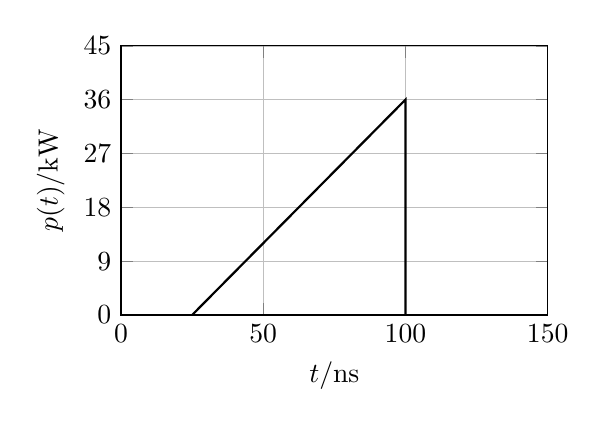
\begin{tikzpicture}
                    \begin{axis}[
                        width=7cm, height=5cm,
                        grid=both,
                        major grid style={line width=.2pt,draw=gray!50},
                        minor grid style={line width=.1pt,draw=gray!20},
                        xlabel={$t$/ns},
                        ylabel={$p(t)$/kW},
                        xmin=0, xmax=150,
                        ymin=0, ymax=45,
                        xtick={0, 50, 100, 150},
                        ytick={0,9, 18, 27, 36, 45},
                    ]
                    % Einschaltverhalten graph
                    \addplot[
                        thick,
                        mark=none,
                        color=black,
                    ] coordinates {
                        (25,0) (100, 36) (100, 0)
                    };
                    \end{axis}
                \end{tikzpicture}
                \caption{Power values for the switch-on process.}
                \label{fig:Power values for the switch-on process}
            \end{subfigure}
            \hfill % Abstand zwischen den Subfiguren
            \begin{subfigure}[t]{0.45\textwidth}
                \centering
                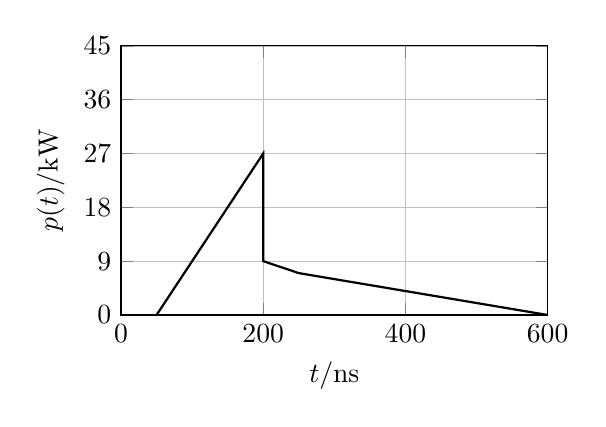
\begin{tikzpicture}
                    \begin{axis}[
                        width=7cm, height=5cm,
                        grid=both,
                        major grid style={line width=.2pt,draw=gray!50},
                        minor grid style={line width=.1pt,draw=gray!20},
                        xlabel={$t$/ns},
                        ylabel={$p(t)$/kW},
                        xmin=0, xmax=600,
                        ymin=0, ymax=45,
                        xtick={0,200, 400, 600},
                        ytick={0,9, 18, 27,36, 45},
                    ]
                    % Ausschaltverhalten graph
                    \addplot[
                        thick,
                        mark=none,
                        color=black,
                    ] coordinates {
                        (50,0) (200, 27) (200, 9) (250, 7) (600,0)
                    };
                    \end{axis}
                \end{tikzpicture}
                \caption{Power values for the switch-off process.}
                \label{fig:Power values for the switch-off process}
            \end{subfigure}
            
            \caption{Switch-on behaviour and switch-off behaviour of $p(t)$}
        \end{solutionfigure}
    \end{solutionblock}


    \subtask{Calculate the switching power loss in the IGBT $P_{\mathrm{VS,T}}$ and in the diode $P_{\mathrm{VS,D}}$.}

\begin{solutionblock}
The switching power loss of the IGBT is dependent on the clock frequency $f_{\mathrm{t}}$ in addition to the switch-on and switch-off power losses.

\begin{equation}
    P_{\mathrm{VS,T}} =  (E_{\mathrm{on,T}} +  E_{\mathrm{off,T}}) \cdot f_{\mathrm{t}} = (\SI {1.35}{\milli\joule} + \SI {3.45}{\milli\joule}) \cdot \SI {25}{\kilo\hertz} = \SI {120}{\watt}
 \end{equation}

 The switching power loss of the diode also depends on the clock frequency $f_{\mathrm{t}}$.
 \begin{equation}
    P_{\mathrm{VS,D}} =  (E_{\mathrm{on,D}} +  E_{\mathrm{off,D}}) \cdot f_{\mathrm{t}} = (\SI {52}{\micro\joule} + \SI {3.45}{\micro\joule}) \cdot \SI {25}{\kilo\hertz} = \SI {7.3}{\watt}
 \end{equation}
\end{solutionblock}

\subtask{ Calculate the conduction losses in the IGBT  $P_{\mathrm{VD,T}}(T)$ and in the diode $P_{\mathrm{VD,D}}(D)$ in
as a function of the relative duty cycle D.}
\begin{solutionblock}
    There are two operating states, one in which the IGBT is closed and another in which it is open. Therefore, the IGBT and diode never carry a current at the same time. This means that the conduction losses of the IGBT only occur when it is switched on.
    \begin{equation}
P_{\mathrm{VD,T}}(T) = u_{\mathrm{CE,on}} I_2  D = \SI {2.5}{\volt}\cdot \SI {30}{\ampere} \cdot D = \SI {75}{\watt} \cdot D
    \end{equation}

    Furthermore, this means that the forward losses of the diode only occur when the IGBT is switched off.
    \begin{equation}
    P_{\mathrm{VD,D}}(T) = u_{\mathrm{f}} I_2 (1-D)= \SI {2.7}{\volt}\cdot \SI {30}{\ampere} \cdot (1-D) = \SI {81}{\watt} \cdot (1-D)
    \end{equation}
\end{solutionblock}

\subtask{Calculate the efficiency $\mu(U_2)$ as a function of the output voltage.}
\begin{solutionblock}
    To determine the efficiency, the general equation $\mu=\frac{P_{\mathrm{disp}}}{P_{\mathrm{sup}}}$ is used.
    \begin{equation}
\mu=\frac{P_{\mathrm{disp}}}{P_{\mathrm{sup}}} = \frac{U_2 I_2}{U_2 I_2 + P_{\mathrm{V,total}}(D)}
    \end{equation}
    $P_{\mathrm{V,total}}(D)$ results from all losses.

    \begin{equation}
P_{\mathrm{V,total}}(D) =  P_{\mathrm{VS,T}} +  P_{\mathrm{VS,D}} + P_{\mathrm{VD,T}}(D) + P_{\mathrm{VD,D}}(D) + P_{\mathrm{V,L}}
\end{equation}

The inductance losses are unknown and have yet to be determined.

\begin{equation}
   P_{\mathrm{V,L}} = R_{\mathrm{CU}} (I_{\mathrm{2}})^2 + P_{\mathrm{V,FE}} = \SI{45}{\mohm} \cdot {(30\ \si{A})^2} + \SI {13}{\watt} = \SI {53.5}{\watt}
    \end{equation}

    $P_{\mathrm{VD,T}}(D)$ and $P_{\mathrm{VD,D}}(D)$ can only be determined in general terms.

    \begin{equation}
P_{\mathrm{VD,T}}(D) + P_{\mathrm{VD,D}}(D) = I_2( u_{\mathrm{CE,on}} D + u_{\mathrm{F}}(D-1)) = D I_2(u_{\mathrm{CE,on}} - u_{\mathrm{F}} ) + I_2 u_{\mathrm{F}}
    \end{equation}

    If you now summarise everything, you come to the solution:
    \begin{equation}
    P_{\mathrm{V,total}}(D) = P_{\mathrm{VS,T}} +  P_{\mathrm{VS,D}} + P_{\mathrm{V,L}} + D I_2(u_{\mathrm{CE,on}} - u_{\mathrm{F}} ) + I_2 u_{\mathrm{F}} =  P_{\mathrm{V,const}} + D I_2 (u_{\mathrm{CE,on}} - u_{\mathrm{F}})
\end{equation}
The value $P_{\mathrm{V,const}}$ is made up of all losses that could be calculated.
\begin{equation}
    P_{\mathrm{V,const}} = \SI {120}{\watt} + \SI {7.3}{\watt} +\SI {53.5}{\watt} + \SI {2.7}{\volt}\cdot\SI {30}{\ampere}
\end{equation}

If these calculations are used in the efficiency as a function of $U_2$, the following result is obtained.

\begin{equation}
    \mu= \frac{U_2 I_2}{U_2 I_2 + P_{\mathrm{V,total}}(D)+D I_2 (u_{\mathrm{CE,on}} - u_{\mathrm{F}})}
\end{equation}
\end{solutionblock}

\subtask{The circuit is now analysed at   $ U_{\mathrm{2}} = \SI{300}{\volt}$. Calculate the total power loss in the IGBT $P_{\mathrm{VT}}$ and in the $P_{\mathrm{VD}}$ diode.}
\begin{solutionblock}
    Firstly, the duty cycle must be determined.
    \begin{equation}
D = \frac{U_2}{U_1} = \frac{\SI{300}{\volt}}{\SI{600}{\volt}} = 0.5
    \end{equation}

    The total power loss of the IGBT is made up of the switching losses and the losses during operation.
    \begin{equation}
    P_{\mathrm{VT}}(D) = u_{\mathrm{CE,on}} I_2 D +  P_{\mathrm{VS,T}} = \SI{2.5}{\volt} \cdot \SI{30}{\ampere} \cdot 0.5 + \SI{120}{\watt} = \SI{157.5}{\watt}
\end{equation}
The total power loss of the diode is made up of the switching losses and the losses during operation.

\begin{equation}
    P_{\mathrm{VD}}(D) = u_{\mathrm{F}} I_2 (1-D) +  P_{\mathrm{VS,D}} = \SI{2.7}{\volt} \cdot \SI{30}{\ampere} \cdot 0.5 + \SI{7.3}{\watt} = \SI{47.8}{\watt}
\end{equation}
\end{solutionblock}
    